\section{Application}
\label{sec:application}

In this section, we demonstrate that \sys{} could significantly improve the performance of realistic applications without modifying the code.
\begin{figure*}[t!]
	\centering
	\begin{minipage}{.31\textwidth}
		\subfloat[Intra-server]{                    
			%\begin{minipage}{0.4\textwidth}
			\centering
			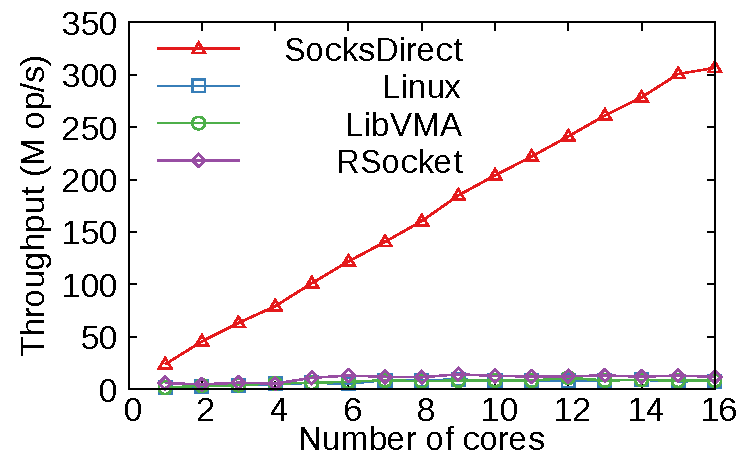
\includegraphics[width=\textwidth]{eval/microbenchmark/corenum-IPC-tput.pdf}
			\label{fig:eval-cornum-ipc}
			%\end{minipage}
		}
		
		\subfloat[Inter-server]{
			%\begin{minipage}{0.4\textwidth}
			\centering 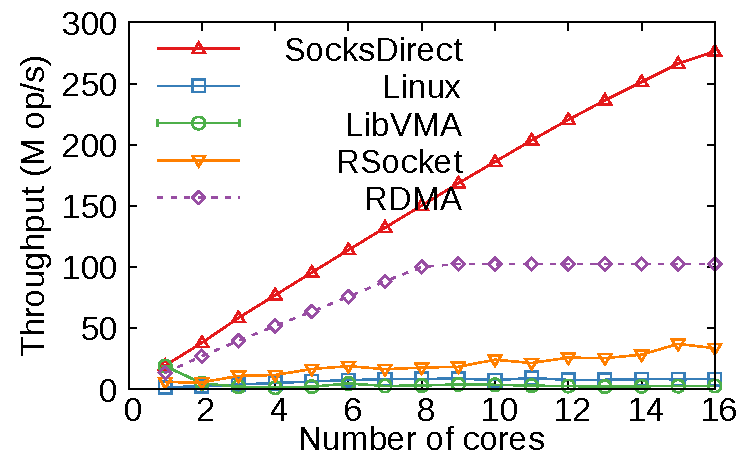
\includegraphics[width=\textwidth]{eval/microbenchmark/corenum-network-tput.pdf}
			\label{fig:eval-cornum-network}
			%\end{minipage}
		}
		\caption{Data transmission throughput with number of cores.}
		\label{fig:eval-corenum-tput}
	\end{minipage}
	\hspace{0.01\textwidth}
	\begin{minipage}{.31\textwidth}
		\centering
		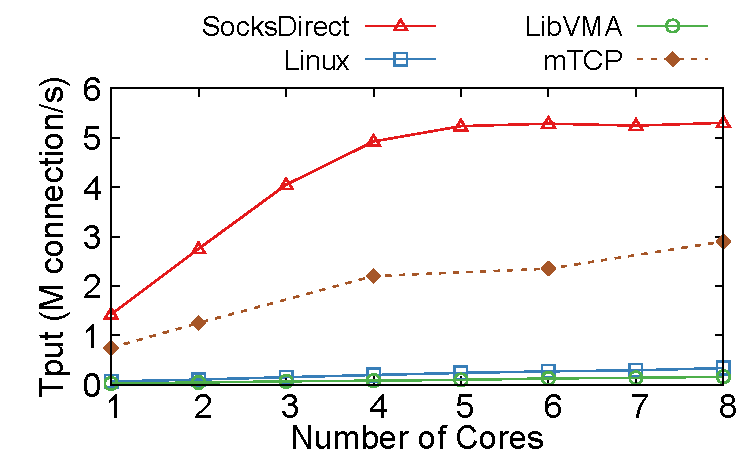
\includegraphics[width=\textwidth]{eval/microbenchmark/conn-setup-tput.pdf}
		\vspace{-10pt}
		\caption{Connection creation throughput with number of cores.}
		\label{fig:eval-conn-setup-tput}
		
		%\begin{minipage}{0.4\textwidth}
		\centering 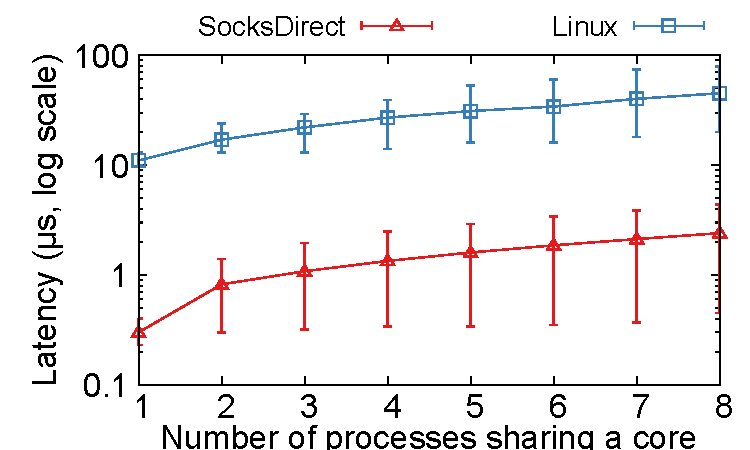
\includegraphics[width=\textwidth]{eval/microbenchmark/sharecore-lat.pdf}
		\vspace{-15pt}
		\label{fig:eval-context-switch}
		\caption{Latency of multiple processes sharing a core.}
		%\end{minipage}
	\end{minipage}
	\hspace{0.01\textwidth}
	\begin{minipage}{.31\textwidth}
		\centering
		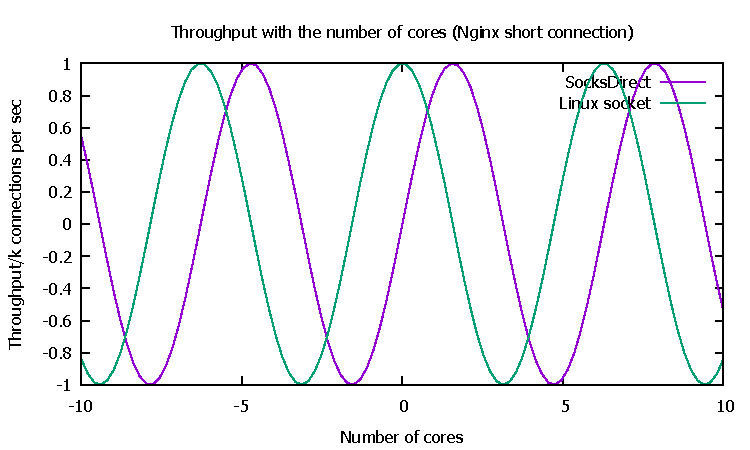
\includegraphics[width=\textwidth]{eval/microbenchmark/nginx-short-tput.pdf}
		\vspace{-15pt}
		\label{fig:eval-nginx-short}
		\caption{Nginx throughput.}
		
		\centering 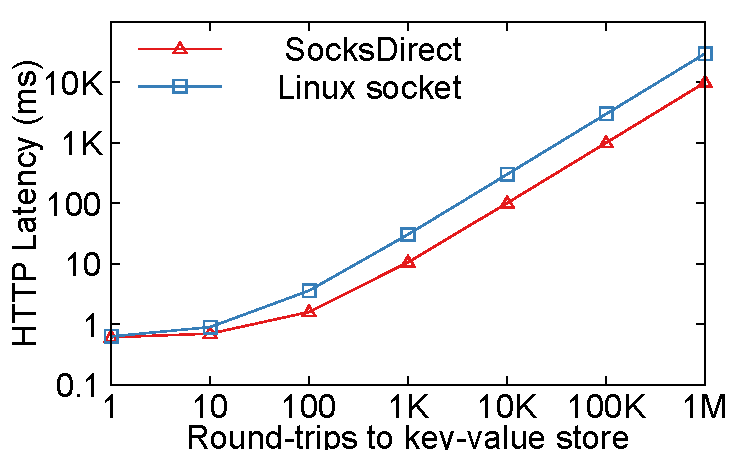
\includegraphics[width=\textwidth]{eval/microbenchmark/nginx-multiround-tput.pdf}
		\vspace{-15pt}
		\caption{HTTP request latency of a web service composed of Nginx, C++ application and memcached.}
		\label{fig:eval-nginx-multiround}
	\end{minipage}
\end{figure*}

\subsection{Network Function}

Network Function Virtualization is prevalent and widely used in modern datacenters. In traditional design, the throughput of Network Functions are highly bounded by the socket in Linux. In this test, we build up chains of Network Functions with different length in one machine. Each Network Function (NF) of chain running as a process and occupies one CPU core. It receives the packet from the predecessor and modifies one byte of the packet, then sends it to the successor of the chain. We compare the performance of \sys{} with Linux socket and ClickOS~\cite{martins2014clickos}. The result illustrates that our design not only could gain throughput up to \RED{data here}, but also highly scalable with the number of cores.

%Network functions~\cite{li2016clicknp}, 

%Scenarios: Firewall (no packet change), NAT (change a packet field), Tunnel endpoint (add/remove packet header, change length)

Metrics: Latency, throughput

\begin{figure}[htpb]
	\centering
	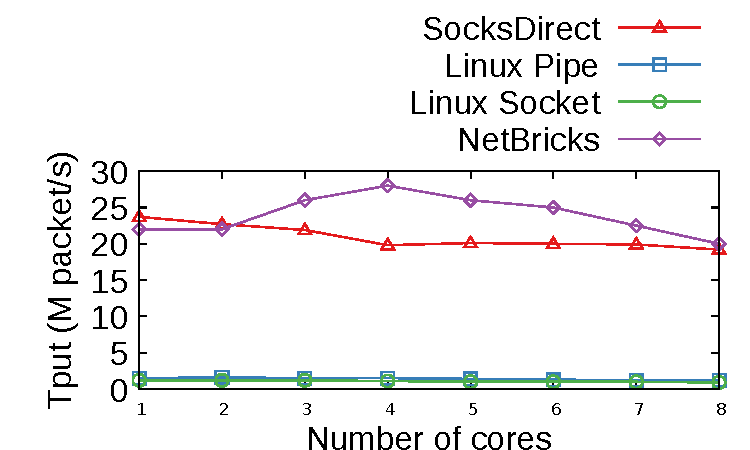
\includegraphics[width=0.33\textwidth]{eval/microbenchmark/nfv-tun-tput.pdf}
	\caption{Throughput of NFV tunnel}
	\label{fig:eval-tun-tput}
\end{figure}



\subsection{Web Application}
For web applications, we conduct experiment for a widely used scenario: one load balancer is connected with the backend webservice, while the webservice accesses the key value store for multiple rounds. The synthetic http traffic is generated and sent to the system.

Figure \ref{fig:eval-nginx-multiround} shows the end-to-end latency with different number of round-trips between the webservice and key value store. As we measured, the Linux socket takes up 69\% of the total time before using our library. Since the intra-server latency of \sys{} is ten times lower that Linux socket, the end-to-end latency of the system with \sys{}  is one third of that with original Linux socket when the number of round trips grows.



%, Nodejs~\cite{nodejs} and memcached~\cite{memcached}

%\begin{itemize}
%	\item Figure~\ref{fig:eval-nginx-short}: Many short-lived connections. %Nginx $\rightarrow$ Nodejs, Nodejs access memcached once.
%	\item Figure~\ref{fig:eval-nginx-multiround}: Each connection, backend %interact extensively. (Nodejs access memcached multiple round trips.)
%\end{itemize}


%\subsection{Real-time Stream Processing}

%Apache Flink~\cite{carbone2015apache} (need to turn off durability on disk)

%Scenario: Word Count (distributed system with one source, two mappers and one reducer)

%Metrics: Latency, throughput

%\subsection{Machine Learning}

%Tensorflow~\cite{abadi2016tensorflow}

%Scenario: (Distributed Tensorflow) Parameter server and worker on a same server.

%Metrics: Time per iteration